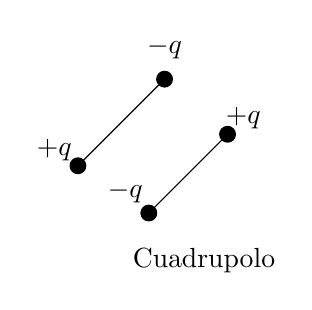
\begin{tikzpicture}
\draw (-1.5,-1) node (v1) {} -- (-0.5,0) node (v2) {};
\draw  [fill](v1) circle (0.1);
\draw  [fill](v2) circle (0.1);
\node at (-1.8,-1) [above]{$-q$};
\node at (-0.3,0.2) {$+q$};

\node at (-0.8,-1.6) {Cuadrupolo};

\draw (-2.4,-0.4) node (v3) {} -- (-1.3,0.7) node (v4) {};
\draw  [fill](v3) circle (0.1);
\draw  [fill](v4) circle (0.1);
\node at (-2.7,-0.2) {$+q$};
\node at (-1.3,1.1) {$-q$};
\end{tikzpicture}